\chapter{Introducció}

L'objectiu principal d'aquest informe és l'estudi de l'aerodinàmica d'un planejador i l'efecte que té sobre ella l'efecte terra. Per tal de poder resoldre el problema plantejat, s'utilitza el mètode numèric de Vortex lattice.

Es comença analitzant l'aerodinàmica de l'ala aïllada per poder estudiar com es troba influenciada pels paràmetres geomètrics, i, un cop determinada la geometria final de l'ala, es procedeix a analitzar l'efecte sòl.

A continuació, s'afegeixen els estabilitzadors vertical i horitzontal i, de nou, se n'estudia els coeficients aerodinàmics. També s'afegeix l'anàlisi de moments. Finalment, es realitza l'anàlisi del planejador complet amb efecte terra.

\begin{figure}[H]
	\centering
	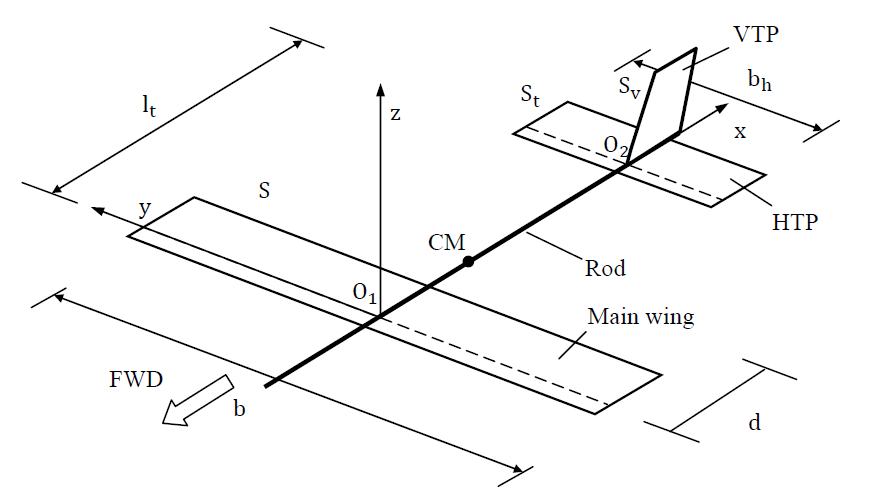
\includegraphics[scale=0.5]{plots/enunciat.png}
	\caption{Esquema del planejador \cite{LizandraDalmases2017a}}
	\label{enunciat}
\end{figure}

L'esquema del planejador, així com els paràmetres geomètrics i els eixos de referència utilitzats, es troben definits en la Figura~\ref{enunciat}. A més, algunes de les relacions entre aquests paràmetres venen fixades per l'enunciat (veure Taula~\ref{tab:Dades}).

\begin{table} [H]
	\centering
	\begin{tabular}{| c | c | c | c |}	
		\hline
		\multicolumn{4}{|c|}{\bfseries Relacions geomètrqiques fixades} \\
		\hline\hline
	\textbf{$S_{t}/S$} & \textbf{$S_{v}/S_{t}$} & \textbf{$l_{t}/\bar{c}$} & \textbf{$A$}\\ \hline 
		$\frac{1}{8}$ & $\frac{2}{3}$ & $4$ & $>6$\\
		\hline	
	\end{tabular}
\caption{Relacions geomètriques fixades} \label{tab:Dades}
\end{table}


A continuació, per tal de definir els paràmetres bàsics de la geometria de l'ala del planejador no establerts, s'ha agafat com a referència l'avió SZD-56 Diana 2 de Diana Sailplanes \cite{Kubrynski2006}. Els valors obtinguts es mostren a la Taula~\ref{tab:WingGeom}.

\begin{table} [h]
	\centering
	\begin{tabular}{| c | c | c | c |}	
		\hline
		\multicolumn{4}{|c|}{\bfseries Paràmetres geomètrics de l'ala} \\
		\hline\hline
	\textbf{$\lambda$} & \textbf{$\Lambda$} & \textbf{$\Gamma$} & \textbf{$A$}\\ \hline 
		$0.3$ & $0$ & $0$ & $26$\\
		\hline	
	\end{tabular}
\caption{Paràmetres geomètrics de l'ala} \label{tab:WingGeom}
\end{table}

Un cop definida la geometria alar, s'ha de definir la geometria dels estabilitzadors tant horitzontal com vertical. Les dimensions escullides es mostren a Taules~ \ref{tab:HSGeom} y \ref{tab:VSGeom}..

\begin{table} [h]
	\centering
	\begin{tabular}{| c | c | c | c | c |}	
		\hline
		\multicolumn{5}{|c|}{\bfseries Estabilitzador horitzontal} \\
		\hline\hline
	\textbf{$\lambda$} & \textbf{$\Lambda$} & \textbf{$\Gamma$} & \textbf{$c_{rh}$} & \textbf{$b_{h}$} \\ \hline
		$0.3$ & $0$ & $0$ & $0.5c_{rW}$ & $0.25b_{w}$\\
		\hline	
	\end{tabular}
\caption{Paràmetres geomètrics de l'estabilitzador horitzontal} \label{tab:HSGeom}
\end{table}

\begin{table} [h]
	\centering
	\begin{tabular}{| c | c | c | c |}	
		\hline
		\multicolumn{4}{|c|}{\bfseries Estabilitzador vertical} \\
		\hline\hline
	\textbf{$\lambda$} & \textbf{$\Lambda$} & \textbf{$\Gamma$} & \textbf{$c_{rV}$}  \\ \hline
		$0.3$ & $0$ & $0$ & $c_{rh}$ \\
		\hline	
	\end{tabular}
\caption{Paràmetres geomètrics de l'estabilitzador vertical} \label{tab:VSGeom}
\end{table}

Per últim, pel que fa als perfils utilitzats, en l'ala s'assumeix un perfil NACA 2412 i en els estabilitzadors vertical i horitzontal, NACA 0009.
